\documentclass[conference,twocolumn]{IEEEtran}
\IEEEoverridecommandlockouts
% The preceding line is only needed to identify funding in the first footnote. If that is unneeded, please comment it out.
\usepackage{cite}
\usepackage{amsmath,amssymb,amsfonts}
\usepackage{float}
\usepackage{algorithmic}
\usepackage{graphicx}
\usepackage{textcomp}
\usepackage{authblk}
\usepackage{pifont}
\usepackage{url} 
\usepackage{pdfpages}
\usepackage{tabularx}
\usepackage{authblk}
\usepackage[utf8]{inputenc}
\usepackage{graphicx}
\graphicspath{ {figures/} }
\usepackage{array}
\def\BibTeX{{\rm B\kern-.05em{\sc i\kern-.025em b}\kern-.08em
   T\kern-.1667em\lower.7ex\hbox{E}\kern-.125emX}}
 
\pagenumbering{roman}

  
 
\begin{document}
\title{\LaTeX\ Biometrics Project Report}

\title{Digital Smile Design}
\author[1]{Ahmed Hossam}
\author[1]{Ahmed Abdelfattah }
\author[1]{Ehab Wahba }
\author[1]{Mo'men Maged}
\author[1]{Mohaned Alaa }
\author[1]{Mostafa Mahmoud}
\affil[1]{Systems and Biomedical Engineering, Cairo University}


\renewcommand\Authands{ and }

\maketitle
\pagestyle{plain}

\section{\textbf{Introduction}}
\textbf{Digital} smile design is a unique dental treatment planning tool that strengthens a dental provider's diagnostic vision, enhances predictability, and improves communication between dental providers and their patients. We've designed a simple software that everyone can use that can detect 5 of the 21 principles of smile design.
\section{\textbf{Methods}}
 The software was made using \textbf{Python} and \textbf{PyQt}. The software can detect the following defects in someone's smile:
\begin{enumerate}
    \item First of all, the mouth is cropped from the original image using 8 point surrounding the mouth using \textbf{Dlib}'s facial landmarks detector.
    \item Teeth Discoloration: using an algorithm that can detect whether the color of the teeth is within the acceptable shades of white.
    \item Midline Shift: using \textbf{Dlib}'s facial landmarks detector, the facial midline can be detected from the eyes center points. Moreover, the dental midline is detected by picking random pixels along the upper teeth with equal distances, then the pixels close to each other are eliminated. In addition, the darkest 3-pixels are chosen, and the distances between each pixel are calculated. If the distances between the 3-pixels are equal, then the dental midline is in the intermediate space between them. Hence, the distance between the dental midline and the facial midline can be calculated.
    \item Diastema: The intermediate distance between the central incisors is calculated by measuring how many dark pixels are between the facial midline and the two central incisors.
    \item Gummy Smile: The ratio between the teeth and gum is calculated in an image by using color masking for the gum and the teeth.
    \item Template Matching: The user can choose between 4 pre-rendered smile templates based on their facial structure.
    
\end{enumerate}

\section{Results and Discussion}
The software was tested on 34 images and had the following results. (The \checkmark means that the principle was detected successfully, and the \ding{55} means that the software showed wrong results).

\begin{figure}[H]
    \centering
    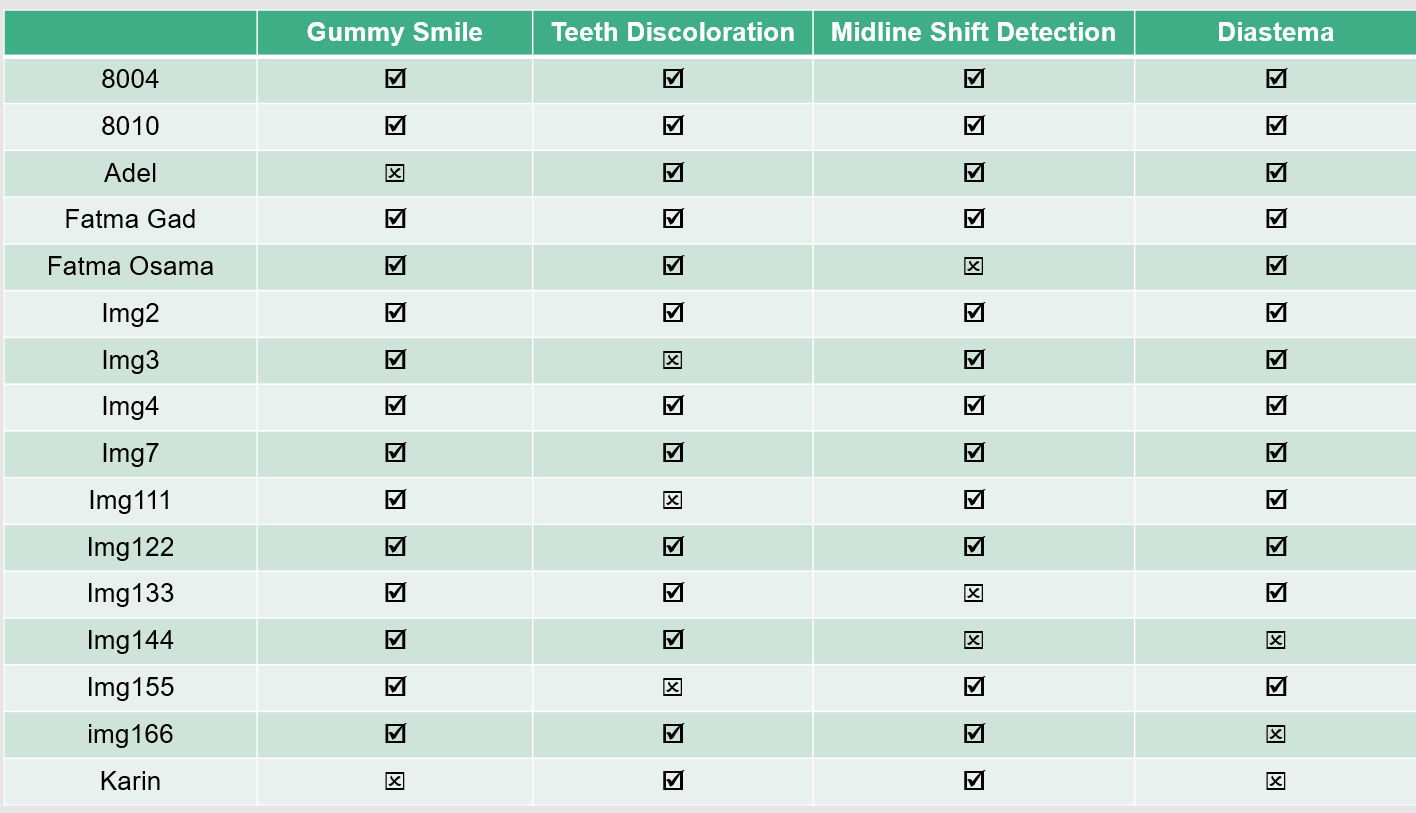
\includegraphics[width=0.55\textwidth]{Screenshot_1.png}
    \caption{Results table 1.}
    \label{fig:my_label}
\end{figure}
\begin{figure}[H]
    \centering
    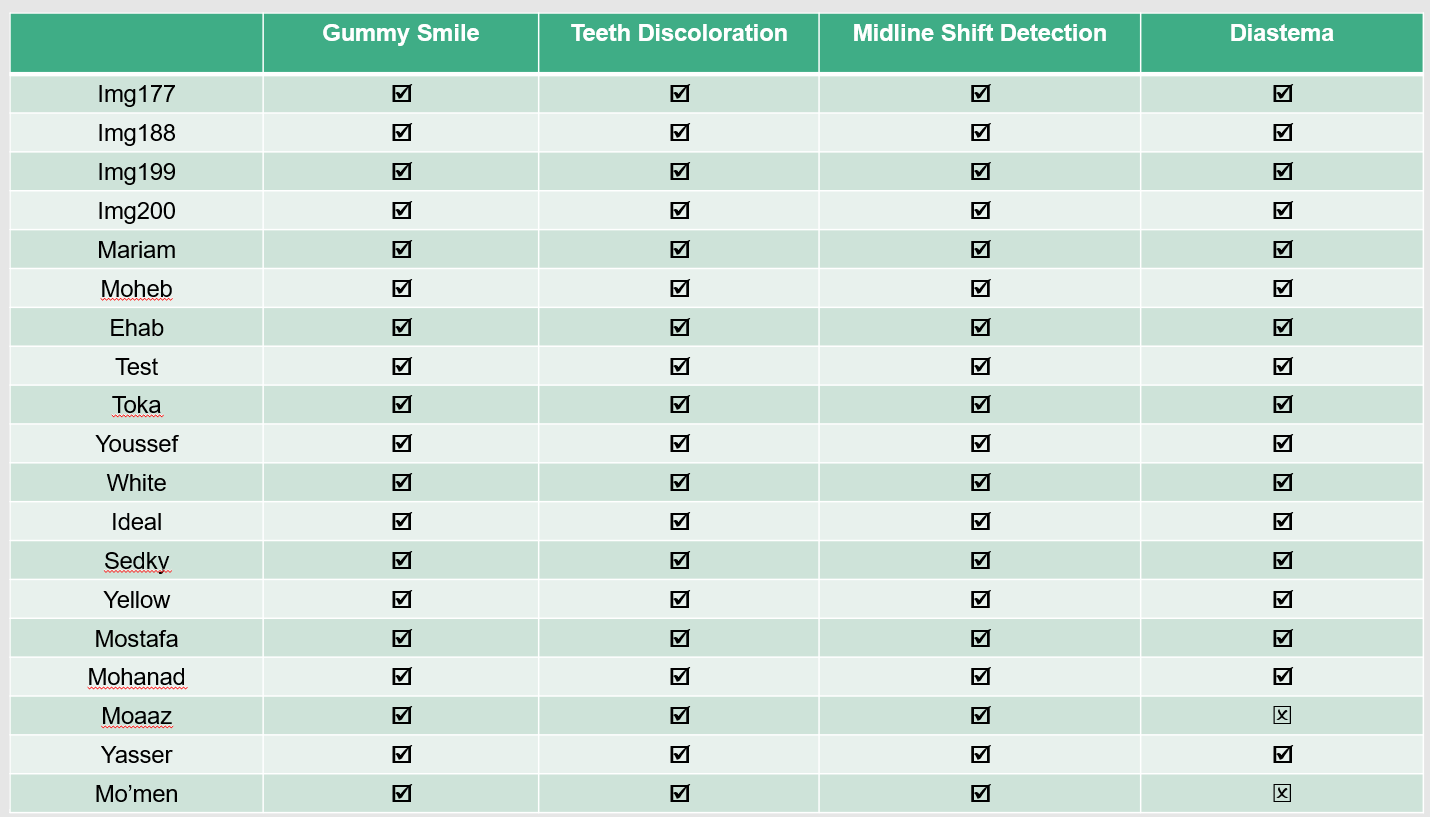
\includegraphics[width=0.55\textwidth]{Screenshot_2.png}
    \caption{Results table 2.}
    \label{fig:my_label}
\end{figure}
\begin{center}
\begin{tabular}{||c c c c||} 
 \hline
 Principle & Successful cases & Accuracy \\ [0.5ex] 
 \hline\hline
 Gummy Smile & 33/35 & 94.3\% \\
 \hline
 Teeth Discoloration & 32/35 & 91.4\% \\
 \hline
 Midline Shift & 30/35 & 85.7\% \\
 \hline
 Diastema & 29/35 & 83\%\\ [1ex] 
\hline
\end{tabular}
\end{center}
\section{Future Work}
The accuracy of the program can be improved by using advanced and improved algorithms to detect the defects. Furthermore, more features can be added to the software such as:
\begin{enumerate}
    \item Horizontal Plane Detection
    \item Golden Proportion Ratio
    \item Vertical Dimension 
    \item Smile at Rest
\end{enumerate}

\section{Conclusion}
Dentists can use the software to diagnose the mentioned defects and use the solutions that the software offers to fix them. Moreover, anyone can use the software as it is has a very simple UI that can detect all of the mentioned defects with the press of a button.

\end{document}